\chapter{Einleitung}
\label{cha:einleitung}
Die nachfolgenden Abschnitte stellen einen Gliederungsvorschlag für ein erstes Kapitel einer in der Forschungsgruppe \gls{CM} am \gls{KIT} erstellten Masterarbeit dar. 

\section{Einführung in das Themengebiet}
Falls der Arbeit ein konkretes Projektszenario zugrunde liegt, ist dieses hier bereits auf hoher Abstraktionsebene einzuführen.

\section{Fragestellungen}
Darstellung der in der Arbeit bearbeiteten Aspekte. Es bietet sich an, in diesem Abschnitt bereits die Grundlage für die Struktur der Gesamtarbeit (im Wesentlichen Kapitel 4 bis 4+n, siehe unten) zu legen.

\section{Beschreibung des Demonstrators}
Der Demonstrator dient dazu, die im vorhergehenden Abschnitt auf konzeptioneller Ebene eingeführten Fragestellungen anhand eines praktischen Beispiels zu verdeutlichen und eine Lösung aufzuzeigen.

\subsection{Zitate}
\label{subsec:zitate}
Der Demonstrator nutzt meist Komponenten, die bereit sin früheren Arbeiten bei \gls{CM} entwickelt wurden.
\begin{quote}
\textit{``A microservice is a cohesive, independent process interacting via messages``}
\end{quote}
\begin{quote}
\textit{``fictive book quote.'', \cite[S.~99]{Be02}}
\end{quote}

\subsection{Grafiken}
Einfügen von Grafiken und referenzieren der Abbildung \ref{fig:lehre}.
\begin{figure}[h]
	\centering
	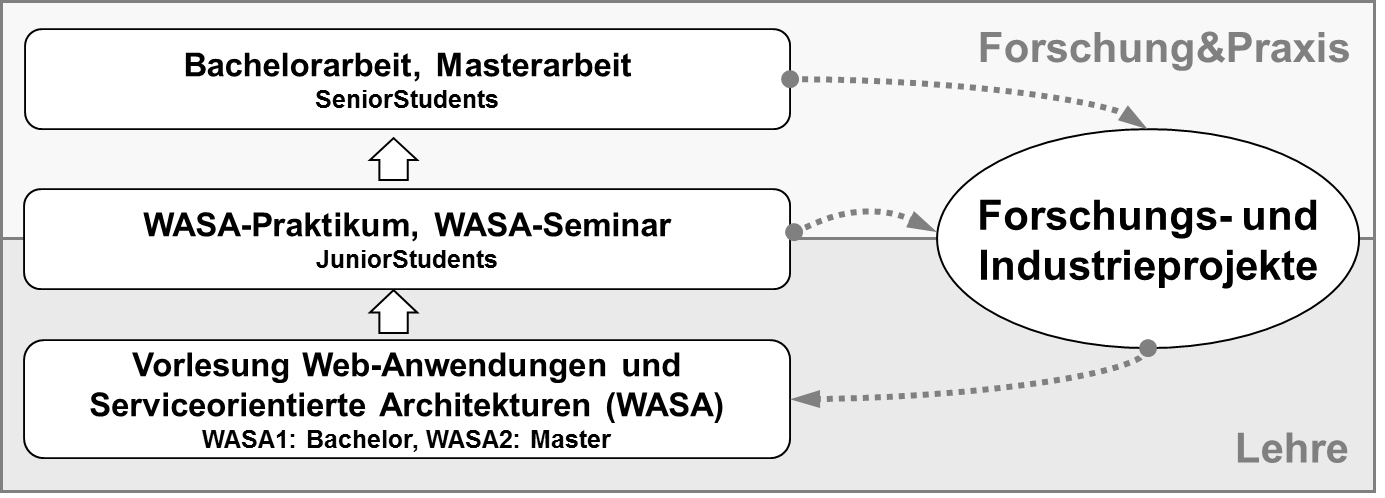
\includegraphics[width=0.8\textwidth]{images/lehre_kreislauf.png}
	\caption{Lehre-Forschung \& Praxis-Kreislauf}
	\label{fig:lehre}
\end{figure}

\begin{table}
	\centering
	\begin{tabular}{ | l | p{7cm} | }
		\hline
		ServiceGroup & Dienstleistung \\
		\hline
		 CoreServiceGroup & Campus-Informationen und Navigation \\
	 	\hline
	 	SCbInfoServiceGroup (SCbSG) & Hörsaal-Informationen für Studierende mit Beeinträchtigung \\
	 	\hline
	 	 StudAdviceTicket (StuSG) & Studierendenberatungs-Anmeldung \\
	 	\hline
	 	WorkspaceServiceGroup (WorSG) & Arbeitsplatz-Suche und -Reservierung \\
	 	\hline
	 	BaMaThesisAdminSG (BaMSG) & Abschlussarbeitenverwaltung \\
	 	\hline
	\end{tabular}
	\caption{ServiceGroups in SmartCampus}
	\label{tab:smartcampus-servicegroups}
\end{table}

\subsection{Quellcode}
\vspace{0.5cm}
\begin{lstlisting}[caption = {Vorlage für eine Story und Szenarien nach BDD}, label = {lst:bdd-stories-szenarien-template}, style = kit-cm, language = Gherkin]
Title (one line describing the story)
 
Narrative:
As a [role]
I want [feature]
So that [benefit]
 
Acceptance Criteria: (presented as Scenarios)
 
Scenario 1: Title
Given [context]
  And [some more context]...
When  [event]
Then  [outcome]
  And [another outcome]...
 
Scenario 2: ...
\end{lstlisting}

\section{Gliederung der Arbeit}
\label{sec:gliederung}
In diesem Kapitel wird der Aufbau der Arbeit in Form der Kapitelstruktur aufgezeigt. Fol-gende Kapitelstruktur wird empfohlen:

\subsection*{Kapitel 2: Grundlagen}

Dieses Kapitel beinhaltet Informationen, die zum grundlegenden Verständnis der Inhalte der Arbeit erforderlich sind. Die Informationen werden weitestgehend "wertfrei" darge-stellt. Beispiele sind:...

\subsection*{Kapitel 3: Stand der Technik}

In dieses Kapitel fließen ganz wesentlich die Ergebnisse der Literaturanalyse ein. Es bietet sich an, die in der Einleitung eingeführte Struktur hier wieder aufzugreifen.

Im Gegensatz zu Kapitel 2 werden die Inhalte dieses Kapitels in einer argumentativen und wertenden Form dargestellt.

\subsection*{Kapitel 4: Inhalt}

Kapitel 4 bis 4+n sind die zentralen konzeptionellen Kapitel der Arbeit, in denen die er-zielten Ergebnisse beschrieben werden.
